\documentclass{article}
\usepackage{graphicx} % Required for inserting images
\usepackage{booktabs} % For better table formatting
\usepackage{array}    % For more flexible table features
\usepackage{placeins} % To control figure placement
\usepackage{float}    % To use the H placement specifier

\title{Analysis of Single Mutants}
\author{Your Name} % Replace with your name
\date{}

% Set graphic path to the directory containing the images
\graphicspath{{/home/hp/nayanika/github/GPX6/figures/}} % Add the path to your images

\begin{document}

\maketitle

\section*{Introduction}
To guide the selection of mutations for directed evolution, a multiple sequence alignment was performed between the human and mouse wild-type protein. This MSA revealed 47 positions that differed between the human and mouse sequences, suggesting potential sites for mutagenesis. In order to prioritize residues for mutagenesis, the distances from the alpha carbon of Cys/Sec49 (active site residue) and the rest of the 46 positions were calculated. Residues were then grouped into distance criteria of <10 Å, 10-15 Å, 15-20 Å, 20-25 Å, 25-30 Å, and 30-35 Å. This distance-based approach allowed us to select residues within different proximity ranges to Cys/Sec49. Grouping residues into distance bins provides a systematic and stochastic way to explore the impact of mutations at varying distances from the target residue (Cys/Sec49). 

To investigate the individual contributions of each residue to the structural and functional differences between the human and mouse proteins, single mutants were generated systematically. Each mutation corresponds to substituting a residue in the mouse protein with its human counterpart, or vice versa, as outlined in the mutation table of 47 residues. This process was conducted one residue at a time to isolate the effects of each mutation.

The mutations were applied by transferring each residue from the mouse sequence to the human sequence and vice versa, ensuring a controlled and systematic approach to mutagenesis. The active site residue, Cys/Sec49, remained a fixed reference point, with all mutations being calculated relative to it. For example, residues such as position 3 (N to K) and position 4 (R to S) involved changes in side-chain polarity or charge, while others, such as position 48 (Y to F), focused on aromatic substitutions. These single-residue changes allow for direct comparisons of the energetic and structural effects of each mutation, enabling us to study how these variations influence activation barriers and overall protein function.

By analyzing the 47 single mutants, we aim to systematically explore the structural transitions and activation energy changes associated with the human-to-mouse and mouse-to-human sequence transformations. This stepwise approach ensures that the contributions of individual residues to protein evolution and function are thoroughly characterized.

\begin{figure}[H]
    \centering
    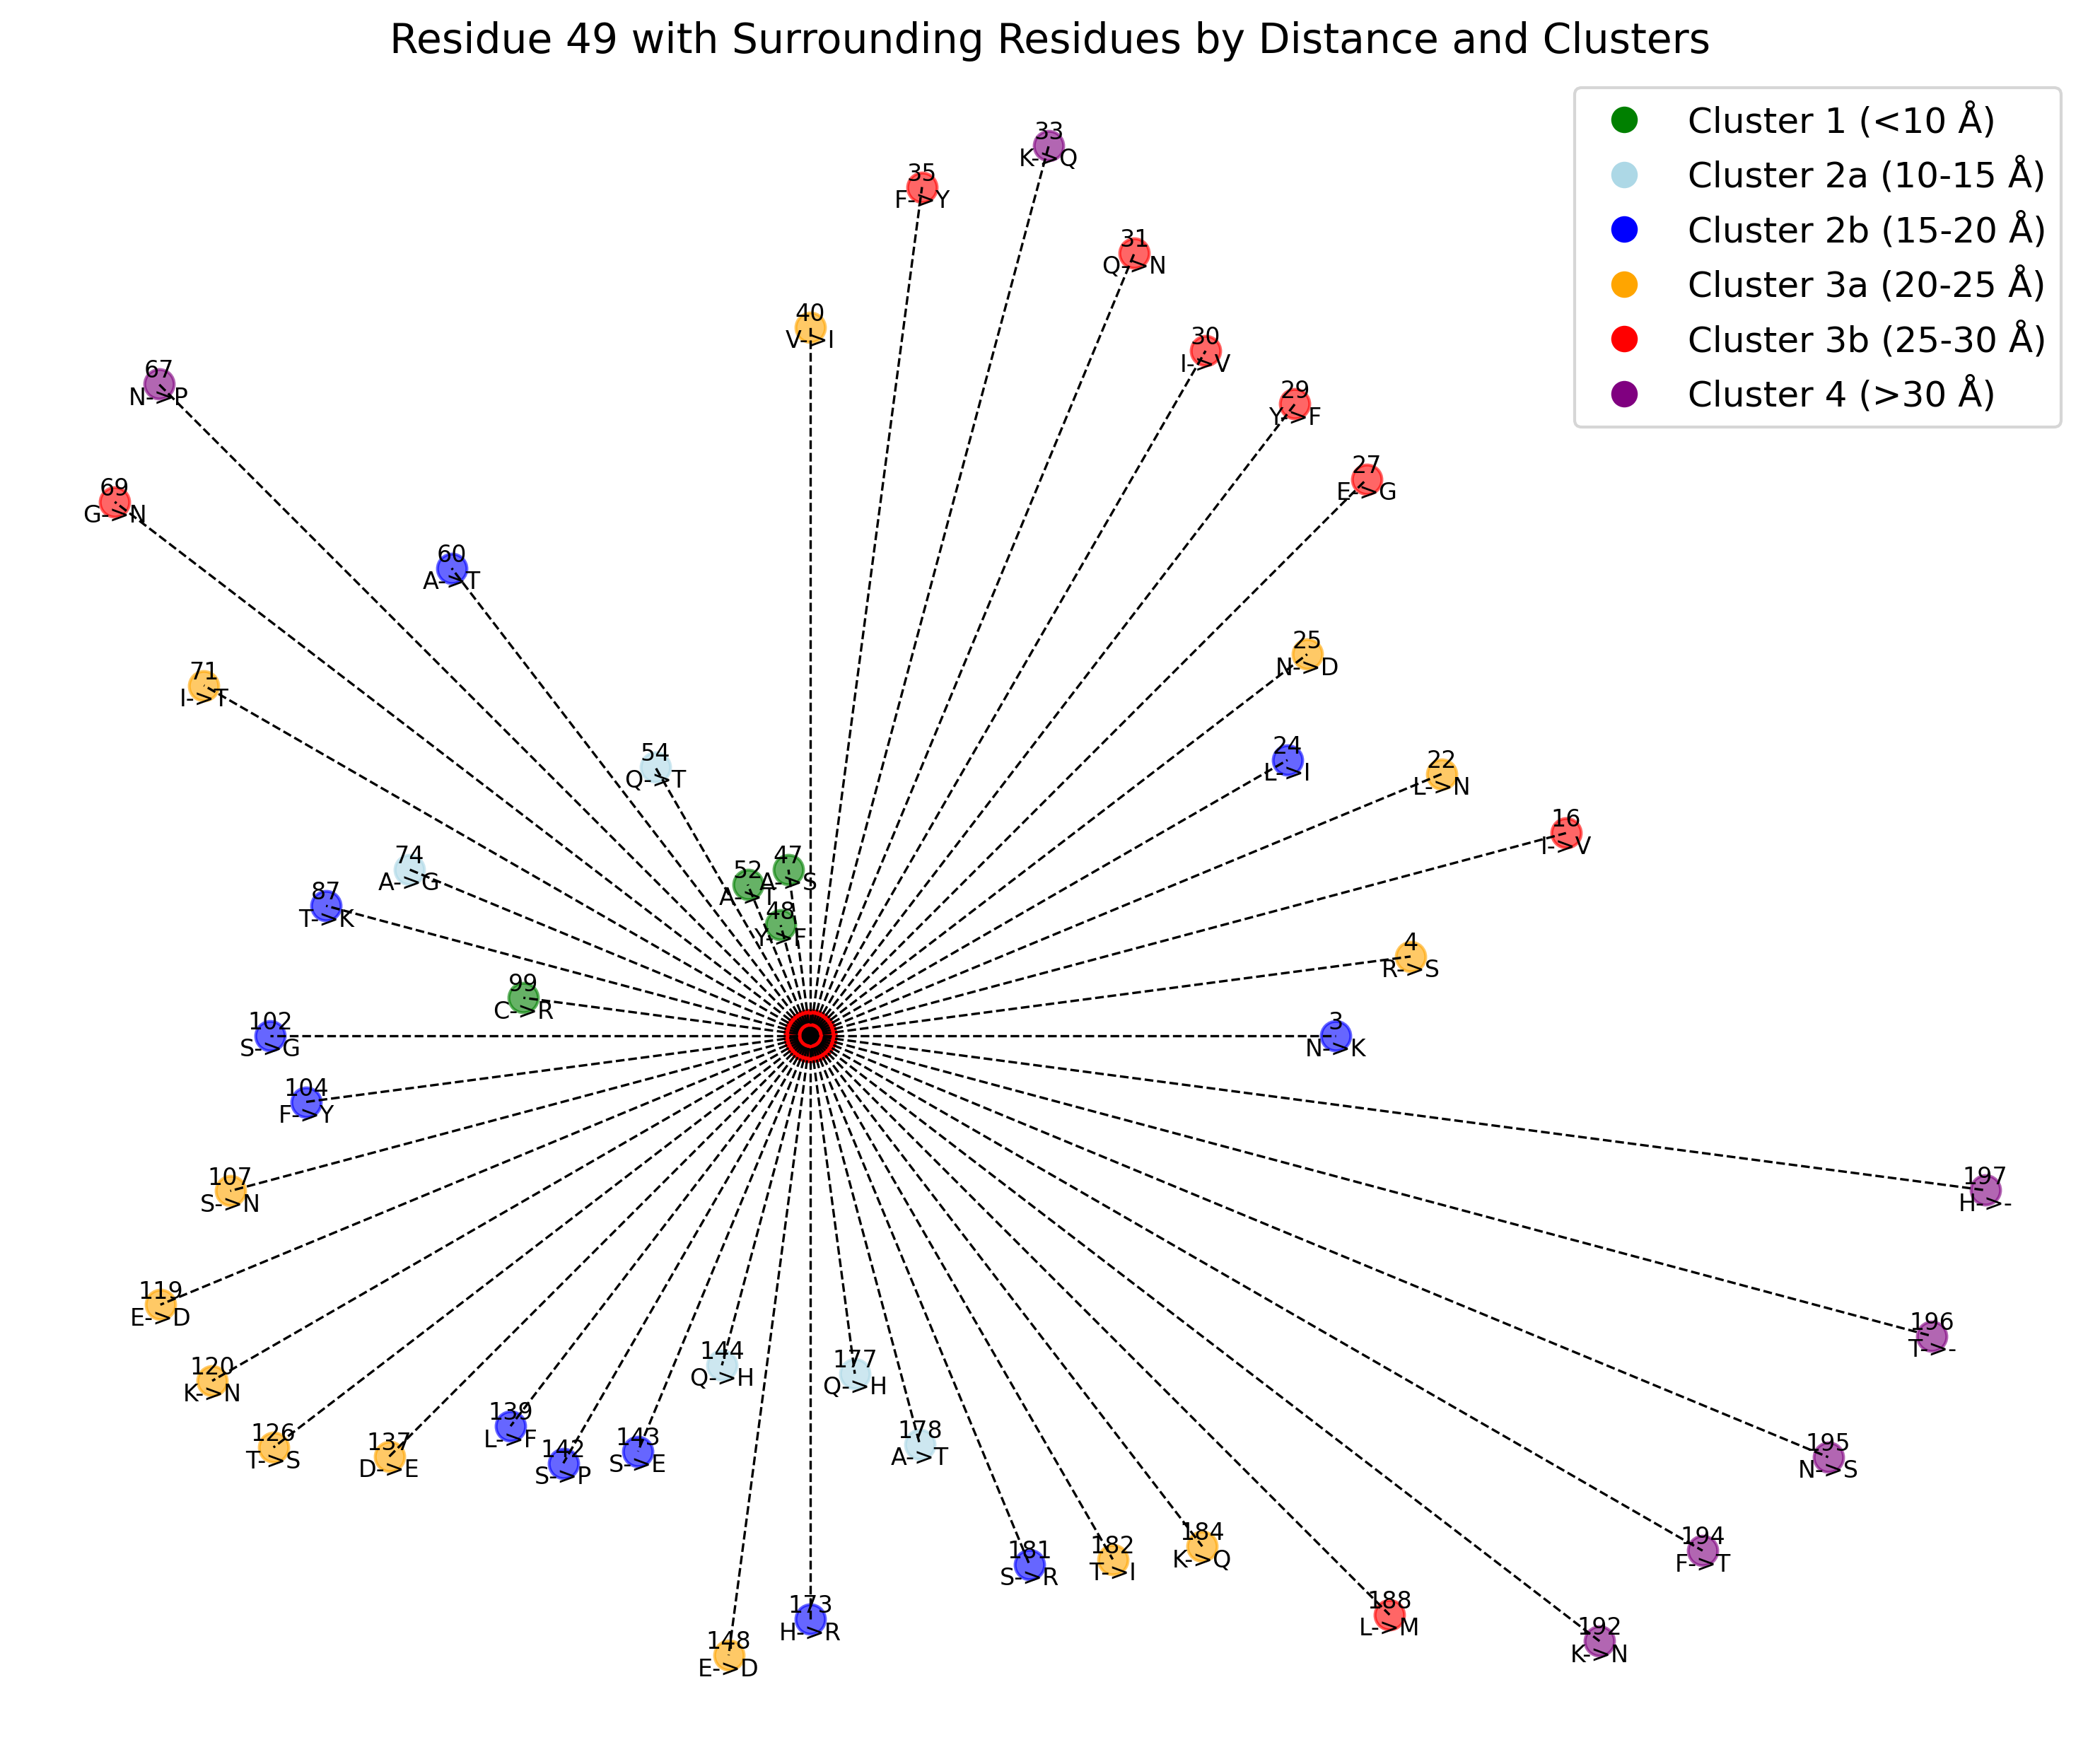
\includegraphics[width=0.8\linewidth]{Residue_human_Distances.png}
    \caption{Distance of residues from the active site for human mutants. The figure highlights proximity of each residue to Cys/Sec49.}
    \label{fig:human_distances}
\end{figure}

\begin{figure}[H]
    \centering
    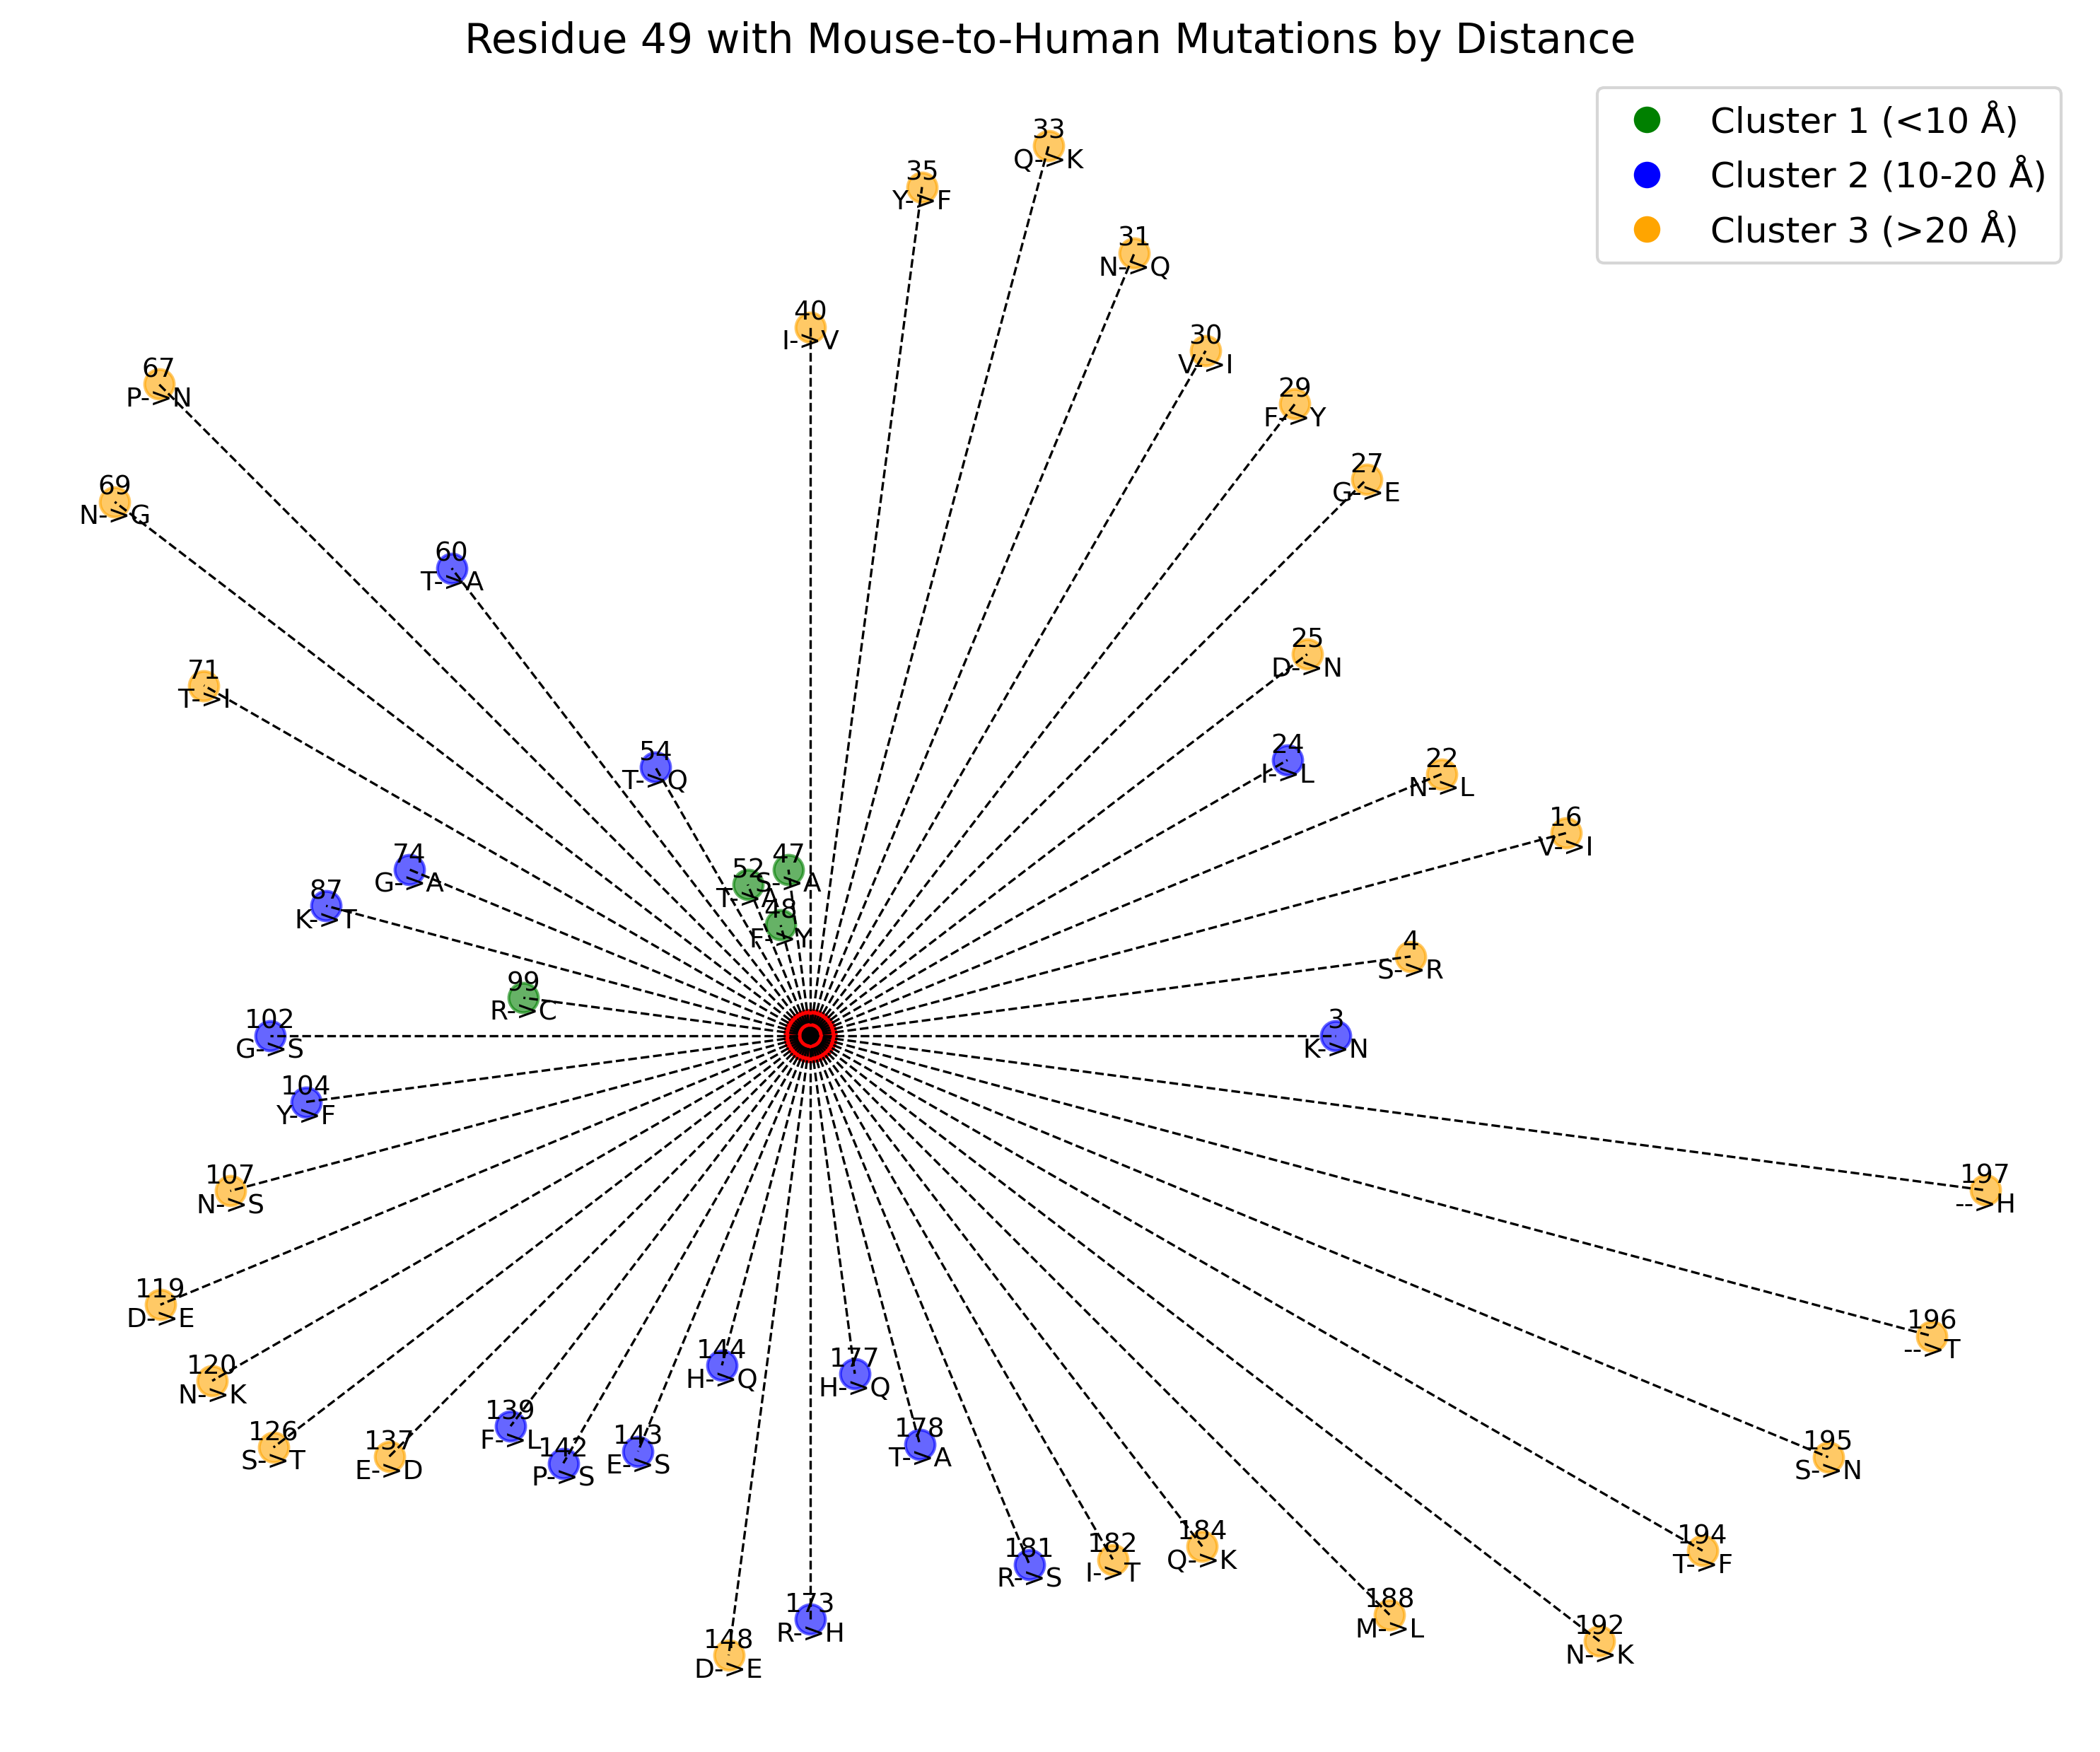
\includegraphics[width=0.8\linewidth]{Residue_mouse_Distances.png}
    \caption{Distance of residues from the active site for mouse mutants. The figure highlights proximity of each residue to Cys/Sec49.}
    \label{fig:mouse_distances}
\end{figure}

\FloatBarrier % Forces all previous figures to appear before this section

\subsection{Clustering the Variants}
The output explains the clustering results of the residues based on their coordinates, which are derived from their distance and free energy values. Here's what the output indicates:

Clusters:

Input Data Preparation
Selected Residues (selected_residues): A list of residues, where each residue is represented as a tuple (position, original_amino_acid, mutated_amino_acid).
Distance Data (distance_dict): A dictionary mapping residue positions to their corresponding distance values.
Free Energy Data (free_energy_dict): A dictionary mapping residue positions to their corresponding free energy values.
2. Filtering and Data Extraction

For each residue, it checks if the position exists in both distance_dict and free_energy_dict.
If valid, it adds a [distance, free_energy] pair to the data list.
The residue position is also recorded in residue_indices.
Finally, the data list is converted into a NumPy array for compatibility with the KMeans algorithm.

3. Clustering Using KMeans
KMeans Initialization: The algorithm is configured to create 2 clusters (n_clusters=2) with a fixed random seed (random_state=42) to ensure reproducibility.
Fitting and Prediction: The fit_predict method clusters the residues based on their distance and free energy.
4. Output Residue Cluster Information
The code prints the cluster assignment for each residue, along with its coordinates (distance, free energy).
5. Distances to Centroids
The script computes the distance of each residue to its assigned cluster centroid using kmeans.transform().
These distances are printed for each residue, providing insight into how close the residue is to the cluster center.

Hydrophobicity Difference=Hydrophobicity of Mutant−Hydrophobicity of Wild-Type
If the amino acid is not in the hydrophobicity scale, a default value of 0 is used.
If the residue position exists in both distance_dict and free_energy_dict, the following data is appended:
Distance (from distance_dict).
Free energy (from free_energy_dict).
Hydrophobicity difference (calculated).
Residue indices are stored for later reference.
The resulting data is converted into a NumPy array.

Clustering Using KMeans
The KMeans algorithm is used with n_clusters=2 to classify residues into two groups based on the 3D feature space:
Distance
Free energy
Hydrophobicity difference
Cluster assignments (clusters) are generated for each residue.

This script:
1. Loads mutation free energy and path data from JSON files.
2. Computes energy differences and rewards for specific node positions.
3. Generates detailed visualizations showing energy rewards along paths, making it easier to analyze trends and relationships between node positions and energy rewards.

DETAILS

- Paths starting with "49" or ending with "33" are selected, and the top 30 entries are retained.
- The filtered data is sorted by energy values in ascending order.

The data is divided into chunks of a maximum of 30 subplots per figure.


\subsection{Visualizing the Clusters}

The following figure illustrates the clustering of mutants based on the distances from the active site and other relevant features. This visualization provides a clear representation of how mutations at different positions affect the protein’s structure and potential function.

\end{document}
